\documentclass[tikz, border=5pt]{standalone}

\begin{document}

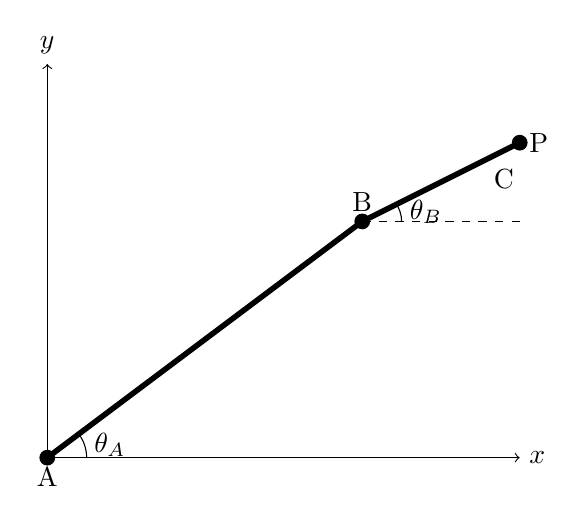
\begin{tikzpicture}

    %% FBD of robotic arm
    % Parametric form

    % Axes
    \draw[->] (0, 0) -- (6, 0) node[right] {$x$};
    \draw[->] (0, 0) -- (0, 5) node[above] {$y$};

    % Arm AB
    \draw[line width=2pt] (0, 0) -- (4, 3);
    \fill (0, 0) circle (0.1);

    % Arm BC
    \draw[line width=2pt] (4, 3) -- (6, 4);
    \fill (4, 3) circle (0.1);

    % Point P
    \fill (6, 4) circle (0.1);

    % Angles
    \draw (0.5, 0) arc (0:36.87:0.5) node[midway, right] {$\theta_A$};
    \draw (4.5, 3) arc (0:36.87:0.4) node[midway, right] {$\theta_B$};

    % Reference
    \draw[dashed] (4, 3) -- (6, 3);

    % Labels
    \node[below] at (0, 0) {A};
    \node[above] at (4, 3) {B};
    \node[above] at (5.8, 3.3) {C};
    \node[right] at (6, 4) {P};

\end{tikzpicture}

\begin{tikzpicture}

    %% FBD of robotic arm

    % Axes
    \draw[->] (0, 0) -- (6, 0) node[right] {$x$};
    \draw[->] (0, 0) -- (0, 5) node[above] {$y$};

    % Arm AB
    \draw[line width=2pt] (0, 0) -- (4, 3);
    \fill (0, 0) circle (0.1);

    % Arm BC
    \draw[line width=2pt] (4, 3) -- (6, 3);
    \fill (4, 3) circle (0.1);

    % Point P
    \fill (6, 3) circle (0.1);

    % Labels
    \node[below] at (0, 0) {A};
    \node[above] at (4, 3) {B};
    \node[above] at (5.5, 2.5) {C};
    \node[right] at (6, 3) {P};

\end{tikzpicture}

\end{document}
